\documentclass{beamer}

\usetheme{CambridgeUS}
\usecolortheme{orchid}

\usepackage[utf8]{inputenc}
\usepackage[T1]{fontenc}

% Paths
\newcommand{\figs}{../figs}
\newcommand{\data}{../data}
\newcommand{\code}{../code}

% URL styles
\usepackage{url}
\urlstyle{sf}

% Units
\usepackage[detect-weight=true, binary-units=true]{siunitx}
\DeclareSIUnit\flop{Flops}

% Math
\usepackage{amsmath}
\usepackage{amssymb}
\usepackage{bm}
\usepackage{nicefrac}
\newcommand{\dif}[1]{{\;\text{d}#1}}

% Graphics
\usepackage{graphicx}
\usepackage{caption}
\usepackage{subcaption}
\graphicspath{{../figs/}}

% Tikz
\usepackage{tikz}
\usetikzlibrary{positioning,shapes,arrows,calc,intersections}
\usepackage{pgfplots}
\usepgfplotslibrary{dateplot}
\pgfplotsset{compat=1.8}

% Colors
\definecolor{darkblue}{HTML}{00688B}
\definecolor{darkgreen}{HTML}{6E8B3D}
\definecolor{cadet}{HTML}{DAE1FF}
\definecolor{salmon}{HTML}{FFB08A}

% Listings
\usepackage{textcomp}
\usepackage{listings}
\lstset{
  keywordstyle=\bfseries\color{orange},
  stringstyle=\color{darkblue!80},
  commentstyle=\color{darkblue!80},
  showstringspaces=false,
  basicstyle=\ttfamily,
  upquote=true,
}
\lstdefinestyle{fortran}{
  language=Fortran,
  morekeywords={for},
  deletekeywords={status},
}
\lstdefinestyle{c}{
  language=C,
  morekeywords={include},
}
\lstdefinestyle{glsl}{
  language=C,
  morekeywords={attribute, vec2, vec3, vec4, varying, uniform, mat2, mat3, mat4},
}
\lstdefinestyle{cuda}{
  language=C,
  morekeywords={__global__, __device__, __host__},
}
\lstdefinestyle{shell}{
  language=bash,
  morekeywords={mkdir, ssh, cmake},
}

% Double hlines
\usepackage{hhline}

% Misc
\usepackage{nth}

\subtitle{TMA4280---Introduction to Supercomputing}

\begin{document}


\title{Multiprocessor systems}
\author{Eivind Fonn}
\institute{SINTEF ICT / NTNU}
\date{December 2015}
\maketitle

\begin{frame}
  \frametitle{Supercomputers at NTNU}
  \begin{center}
    \scalebox{0.8}{
      \bgroup\def\arraystretch{1.2}
\begin{tabular}{llrlr}
  \hline
  Year & System & Processors & Type & $\SI{}{\giga\flop}$ \\
  \hhline{=====}
  1986--1992 & Cray X-MP & 2 & Vector & 0.5 \\
  1992--1996 & Cray Y-MP & 4 & Vector & 1.3\\
  1995--2003 & Cray J90     & 8 & Vector & 1.6 \\
  1992--1999 & Intel Paragon & 56 & MPP & 5.0\\
  1996--2003 & Cray T3E & 96 & MPP & 58\\
  2000--2001 & SGI O2 & 160 & ccNUMA & 100\\
  2001--2008 & SGI O3 & 898 & ccNUMA & 1000\\
  2006--2011 & IBM P5+ & 2976 & Distributed SMP & 23500\\
  2012--     & SGI Altix ICE X & 23040 & Distributed SMP & 497230 \\
  \hline
\end{tabular}
\egroup

    }
  \end{center}
\end{frame}

\begin{frame}
  \frametitle{Supercomputers}
  \begin{itemize}
  \item 70's--80's: vector processors; \\
    one or a few expensive, custom-made chips.
  \item 80's--: MPP systems; \\
    many processors; standard micro-processors.
  \item Current trend: multicore systems; \\
    heterogeneous computing.
  \end{itemize}
\end{frame}

\begin{frame}
  \frametitle{Multi-processor systems}
  Challenges:
  \begin{itemize}
  \item communication between processors \\
    (memory access, programming models);
  \item computational methods or algorithms;
  \item scalability (hardware and algorithms);
  \item large volumes of data (storage and visualization).
  \end{itemize}
\end{frame}

\begin{frame}
  \frametitle{Shared memory access}
  \begin{center}
    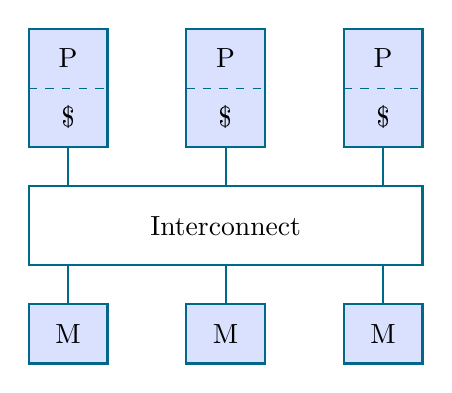
\begin{tikzpicture}[scale=0.5]
  \foreach \i in {0,4,8}
  {
    \draw[darkblue, fill=cadet, thick] (\i,10) rectangle (\i+2,7);
    \draw[darkblue, very thin, dashed] (\i,8.5) -- (\i+2,8.5);
    \draw[darkblue, fill=cadet, thick] (\i,3) rectangle (\i+2,1.5);
    \draw[darkblue, thick] (\i+1,7) -- (\i+1,6);
    \draw[darkblue, thick] (\i+1,3) -- (\i+1,4);
    \node at (\i+1,9.25) {P};
    \node at (\i+1,7.75) {\$};
    \node at (\i+1,2.25) {M};
  }
  \draw[darkblue, thick] (0,6) rectangle (10,4);
  \node at (5,5) {Interconnect};
\end{tikzpicture}

  \end{center}
\end{frame}

\begin{frame}
  \frametitle{Distributed memory access}
  \begin{center}
    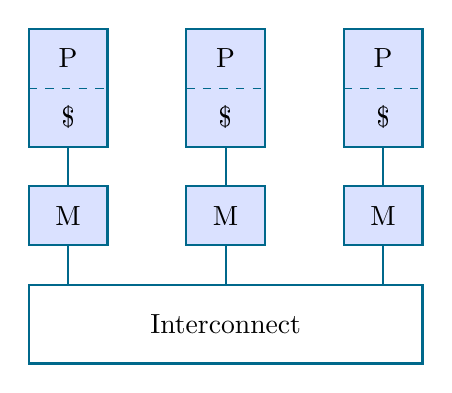
\begin{tikzpicture}[scale=0.5]
  \foreach \i in {0,4,8}
  {
    \draw[darkblue, fill=cadet, thick] (\i,10) rectangle (\i+2,7);
    \draw[darkblue, very thin, dashed] (\i,8.5) -- (\i+2,8.5);
    \draw[darkblue, fill=cadet, thick] (\i,6) rectangle (\i+2,4.5);
    \draw[darkblue, thick] (\i+1,7) -- (\i+1,6);
    \draw[darkblue, thick] (\i+1,3.5) -- (\i+1,4.5);
    \node at (\i+1,9.25) {P};
    \node at (\i+1,7.75) {\$};
    \node at (\i+1,5.25) {M};
  }
  \draw[darkblue, thick] (0,1.5) rectangle (10,3.5);
  \node at (5,2.5) {Interconnect};
\end{tikzpicture}

  \end{center}
\end{frame}

\begin{frame}
  \frametitle{Shared memory: uniform access}
  This is called a \emph{symmetric multi-processor}. Examples: bus-based,
  switch-based and crossbar organizations. Challenges: cache coherency and cost.
  \begin{center}
    \scalebox{0.6}{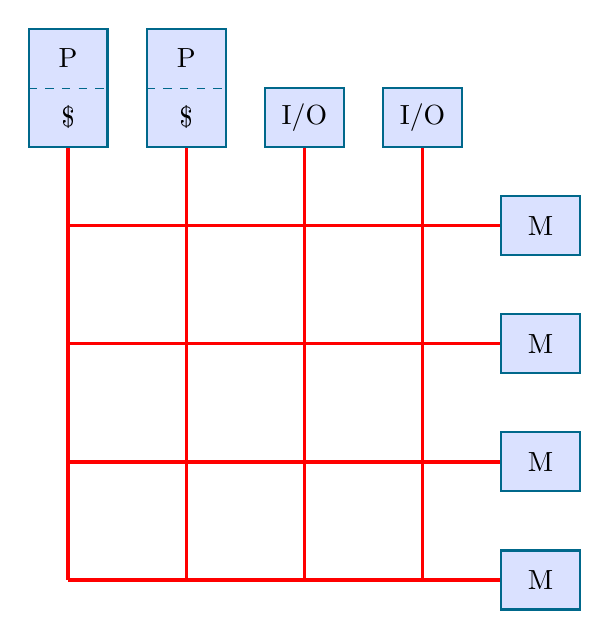
\begin{tikzpicture}[scale=0.5]
  \foreach \i in {0,3,6,9}
  {
    \draw[red, very thick] (0,\i) -- (11,\i);
    \draw[red, very thick] (\i,0) -- (\i,11);

    \draw[darkblue, fill=cadet, thick] (11,\i+.75) rectangle (13,\i-.75);
    \node at (12,\i) {M};
  }

  \foreach \i in {0,3}
  {
    \draw[darkblue, fill=cadet, thick] (\i-1,14) rectangle (\i+1,11);
    \draw[darkblue, very thin, dashed] (\i-1,12.5) -- (\i+1,12.5);
    \node at (\i,13.25) {P};
    \node at (\i,11.75) {\$};
  }

  \foreach \i in {6,9}
  {
    \draw[darkblue, fill=cadet, thick] (\i-1,12.5) rectangle (\i+1,11);
    \node at (\i,11.75) {I/O};
  }
\end{tikzpicture}
}
  \end{center}
\end{frame}

\begin{frame}
  \frametitle{Shared memory: non-uniform access}
  This is called NUMA or ccNUMA (\emph{cache-coherent non-uniform memory
    access}). Example: Several SMPs connected with a high-speed low-latency
  network. Each SMP has uniform memory access internally.
  \begin{center}
    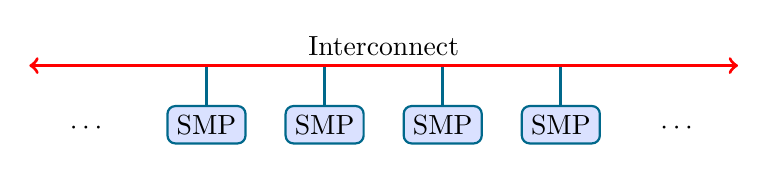
\begin{tikzpicture}[
  scale=0.5,
  block/.style={
    minimum height=2,
    minimum width=2,
    shape=rectangle,
    fill=cadet,
    draw=darkblue,
    rounded corners=1mm,
    text centered,
    thick,
  }
  ]
  \foreach \i in {4.5, 7.5, 10.5, 13.5} {
    \node[block, anchor=north] at (\i,-1) {SMP};
    \draw[very thick, darkblue] (\i,0) -- (\i,-1);
  }
  \draw[red, very thick, <->] (0,0) -- (18,0);
  \node[anchor=south] at (9,0) {Interconnect};
  \node[anchor=north] at (16.5,-1.2) {$\cdots$};
  \node[anchor=north] at (1.5,-1.2) {$\cdots$};
\end{tikzpicture}

  \end{center}
\end{frame}

\begin{frame}
  \frametitle{Distributed memory systems}
  Only the local address space is available to each processor. Data from other
  processors are only available through explicit message-passing.
  \begin{center}
    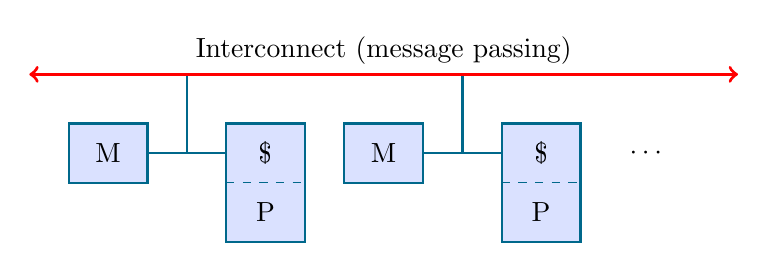
\begin{tikzpicture}[scale=0.5]
  \foreach \i in {3, 10}
  {
    \draw[darkblue, thick] (\i+1,-2) -- (\i+1,0);
    \draw[darkblue, thick] (\i,-2) -- (\i+2,-2);

    \draw[darkblue, fill=cadet, thick] (\i-2,-2.75) rectangle (\i,-1.25);
    \node at (\i-1,-2) {M};

    \draw[darkblue, fill=cadet, thick] (\i+2,-1.25) rectangle (\i+4,-4.25);
    \draw[darkblue, very thin, dashed] (\i+2,-2.75) -- (\i+4,-2.75);
    \node at (\i+3,-2) {\$};
    \node at (\i+3,-3.5) {P};
  }

  \draw[red, very thick, <->] (0,0) -- (18,0);
  \node[anchor=south] at (9,0) {Interconnect (message passing)};
  \node[anchor=west] at (15,-2) {$\cdots$};
\end{tikzpicture}

  \end{center}
\end{frame}

\begin{frame}
  \frametitle{Network topology}
  Examples: 2D mesh or toroid. Vilje is an eight-dimensional hyper-cube (!).
  \begin{center}
    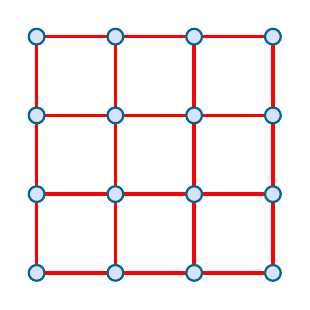
\begin{tikzpicture}
  \foreach \i in {0,...,3} {
    \draw[very thick, red] (\i,0) -- (\i,3);
    \draw[very thick, red] (0,\i) -- (3,\i);
  }
  \foreach \i in {0,...,3} {
    \foreach \j in {0,...,3} {
      \draw[thick, darkblue, fill=cadet] (\i,\j) circle (0.1);
    }
  }
\end{tikzpicture}

    \qquad
    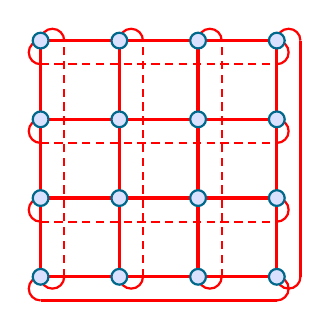
\begin{tikzpicture}
  \foreach \i in {0,...,3} {
    \draw[very thick, red] (\i,0) -- (\i,3);
    \draw[very thick, red] (0,\i) -- (3,\i);
  }
  \foreach \i in {0,...,3} {
    \draw[thick, red] (\i,0) arc (180:360:0.15);
    \draw[thick, red] (\i+0.3,3) arc (0:180:0.15);
    \draw[thick, red] (0,\i) arc (90:270:0.15);
    \draw[thick, red] (3,\i-0.3) arc (270:450:0.15);
  }
  \foreach \i in {0,...,2} {
    \draw[thick, red, densely dashed] (\i+0.3,0) -- (\i+0.3,3);
    \draw[thick, red, densely dashed] (0,\i+0.7) -- (3,\i+0.7);
  }
  \draw[thick, red] (3.3,0) -- (3.3,3);
  \draw[thick, red] (0,-0.3) -- (3,-0.3);
  \foreach \i in {0,...,3} {
    \foreach \j in {0,...,3} {
      \draw[thick, darkblue, fill=cadet] (\i,\j) circle (0.1);
    }
  }
\end{tikzpicture}

  \end{center}
\end{frame}

\begin{frame}
  \frametitle{The current supercomputer at NTNU}
  Based on the Intel Sandy Bridge microprocessor, an octa-core chip (image
  shows the quad-core version)
  \begin{center}
    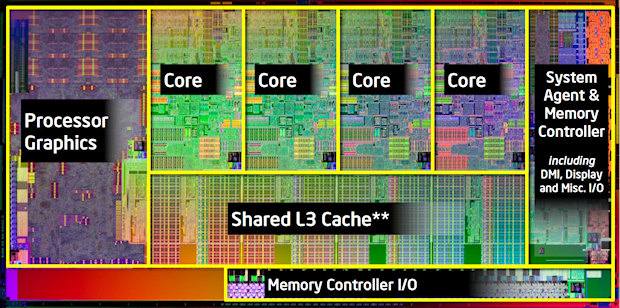
\includegraphics[width=9.5cm]{sandy}
  \end{center}
\end{frame}

\begin{frame}
  \frametitle{The current supercomputer at NTNU}
  Intel Sandy bridge E5-2670:
  \begin{itemize}
  \item An octa-core chip (8 physical processing cores)
  \item Caches and memory:
    \begin{itemize}
    \item private L1 cache (32kB instruction+32kB data) 3 clocks;
    \item private L2 cache (256kB) 8 clocks;
    \item shared L3 cache (20MB) $\sim$ 30 clocks (could not find info);
    \item main memory (32GB) $\sim$ 150 clocks (could not find info).
    \end{itemize}
  \item FMA capable AVX unit, meaning 8 Flop per cycle, SSE 4.x.
  \item Simultaneous multi-threading (SMT): Intel calls this ``hyperthreading'':
    each processor core can handle two instruction streams at the same time.
    Problem: Shared SIMD units.
  \end{itemize}
\end{frame}

\begin{frame}
  \frametitle{A node: two E5-2670 chips}
  \begin{center}
    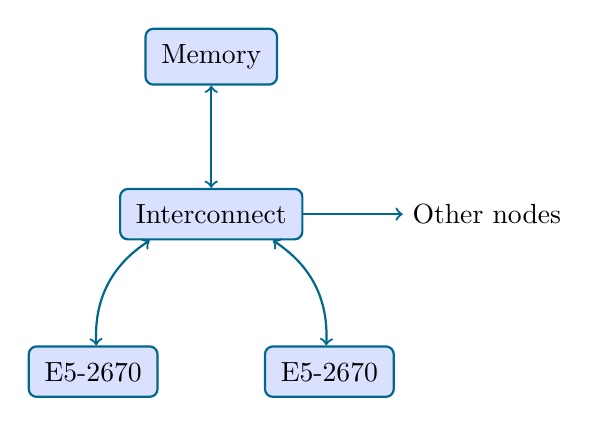
\begin{tikzpicture}[
      proc/.style={
        inner sep=2mm,
        shape=rectangle,
        rounded corners=1mm,
        draw=darkblue,
        fill=cadet,
        thick,
      }]
      \node[proc] (p1) at (0,0) {E5-2670};
      \node[proc] (p2) at (3,0) {E5-2670};
      \node[proc] (ict) at (1.5,2) {Interconnect};
      \node[proc] (mem) at (1.5,4) {Memory};
      \node (nodes) at (5,2) {Other nodes};
      \draw[<->, thick, darkblue] (p1) edge[bend left] (ict);
      \draw[<->, thick, darkblue] (p2) edge[bend right] (ict);
      \draw[<->, thick, darkblue] (ict) -- (mem);
      \draw[->, thick, darkblue] (ict) -- (nodes);
    \end{tikzpicture}
  \end{center}
\end{frame}

\begin{frame}
  \frametitle{Key data}

  Vilje:
  \begin{itemize}
  \item 1440 nodes or 23040 physical cores;
  \item 16-core shared memory within a single node;
  \item distributed memory across nodes;
  \item 394 TB storage.
  \item 8.6GB/s aggregated bandwidth.
  \end{itemize}

  Programming models:
  \begin{itemize}
  \item shared memory programming model (OpenMP) within a node;
  \item message passing (MPI) across nodes;
  \item also possible: message passing within a single node;
  \item also possible: both models within the same program.
  \end{itemize}
\end{frame}

\end{document}

